\documentclass[a4paper,11pt]{article}
\usepackage{amsmath}
\usepackage{graphicx}
\usepackage{hyperref}
\usepackage{geometry}
\usepackage{listings}
\geometry{margin=1in}
\hypersetup{
    colorlinks=true,
    linkcolor=blue,
    urlcolor=blue
}
\usepackage{float}

\title{REPORT: Mixture of Experts (MoE) Model for Image Processing}
\author{Carlos Garcia}
\date{\today}

\begin{document}

\maketitle

\section{Introduction}
Mixture of Experts (MoE) models have gained significant attention due to their ability to combine multiple specialized models (``experts") to improve the performance of deep learning architectures. Although MoE models are traditionally applied in natural language processing (NLP) \cite{shazeer2017outrageously}, this report explores their adaptation to image processing tasks. Specifically, we implement and evaluate a transformer-based MoE model for image classification.

\section{Mixture of Experts (MoE) Overview}
MoE is a concept where different ``experts" are selected dynamically based on the input data. In the MoE architecture, each input is routed to a subset of these experts, typically using a gating mechanism, ensuring that only the most relevant experts are utilized at any given time. This approach not only reduces computational cost, but also increases flexibility and specialization in the model \cite{huggingfaceMixtureExperts}.

For this project, the transformer architecture \cite{vaswani2017attention} is adapted, where the feed-forward layers in the transformer blocks are replaced with expert layers. The MoE mechanism for image processing introduces unique challenges compared to its application in NLP, particularly in handling the two-dimensional structure of images.

\section{Model Implementation}
The model is implemented in PyTorch \cite{pytorch}, utilizing the MoE design to replace the feed-forward layers in a transformer encoder block with specialized expert layers. We use the MNIST dataset \cite{deng2012mnist}, which is widely used to benchmark image classification models. The implementation consists of:
\begin{itemize}
    \item \textbf{Experts}: Each expert is a simple network composed of two linear layers with a GELU activation function \cite{hendrycks2020gaussian}.
    \item \textbf{Gating Mechanism}: A learned linear layer is used to route input data to a selected subset of experts based on the top-k gating strategy.
    \item \textbf{Transformer Architecture}: A traditional transformer encoder is employed, where MoE layers are integrated. The transformer processes image patches extracted from the MNIST dataset as in the Vision Transformer (ViT) \cite{dosovitskiy2020image}.
    \item \textbf{Training Pipeline}: The model is trained using the Adam optimizer and a standard cross-entropy loss function. The training pipeline is tracked using MLFlow \cite{mlflow} and DAGsHub \cite{dagshub}.
    \item \textbf{Hyperparameter Tuning}: Key hyperparameters such as the number of experts, top-k selection, patch size, and expert placement are tuned to optimize the model's performance.
\end{itemize}

% \begin{lstlisting}[language=Python]
% class MoELayer(nn.Module):
%     def __init__(self, num_experts, d_model, d_ff, k=2):
%         super().__init__()
%         self.num_experts = num_experts
%         self.k = k
%         self.gate = nn.Linear(d_model, num_experts)
%         self.experts = nn.ModuleList([Expert(d_model, d_ff) for _ in range(num_experts)])

%     def forward(self, x):
%         batch_size, seq_len, d_model = x.shape
%         gate_outputs = self.gate(x)
%         top_k_gates, top_k_indices = torch.topk(gate_outputs, self.k, dim=-1)
%         top_k_gates = torch.softmax(top_k_gates, dim=-1)
%         expert_outputs = torch.zeros_like(x).unsqueeze(-2).repeat(1, 1, self.k, 1)
%         for i in range(self.k):
%             idx = top_k_indices[:, :, i]
%             expert_outputs[:, :, i, :] = torch.stack([self.experts[idx[b, s]](x[b, s]) for b in range(batch_size) for s in range(seq_len)]).view(batch_size, seq_len, -1)
%         output = torch.sum(top_k_gates.unsqueeze(-1) * expert_outputs, dim=2)
%         return output
% \end{lstlisting}

\section{Training and Experimentation}
Given the constraints on computational resources, training time was a critical consideration during the experiments. The process was divided into five key stages:

\begin{itemize}
    \item \textbf{Number of Experts and Top-k Selection}: 
    We evaluated combinations of parameters $num\_experts = [2, 4, 8, 16, 32]$ and $top-k = [2, 4, 8]$. The optimal balance between accuracy and computational cost was achieved with $num\_experts = 4$ and $top-k = 2$ (Figure \ref{fig:experts_topk}), which served as the base configuration for subsequent experiments.

    % ----------------
    
    \item \textbf{Patch Size}: The impact of patch size on model performance was systematically assessed. Although smaller patch sizes allow the model to capture finer details, they also significantly increase computational costs and may hinder convergence. We tested patch sizes of $patch\_size = [4, 8, 16, 32]$. The best trade-off between accuracy and computational cost was found with a patch size of $16 \times 16$ (Figure \ref{fig:patch_size}).

    % ----------------

    \item \textbf{Number of Layers and Expert Placement}: Initial tests were performed on the number of layers, with values $n\_layers = [2, 3, 4, 5]$. The optimal balance was found with $n\_layers = 3$. Subsequently, we evaluated the placement of experts within the transformer layers, testing $expert\_placement = ['all', [0], [1], [2], [0, 2]]$. The best results were obtained when the experts were placed in the middle of the transformer layers ($expert\_placement = [[2]]$) (Figure \ref{fig:layers_placement}). Generally, the model performed better when experts were neither too early nor too late in the transformer layers, and not in all layers.

    % ----------------

    \item \textbf{Learning Rate}: The learning rate was fine-tuned to identify the optimal value for the model. We tested $learning\_rate = [0.01, 0.005, 0.001, 0.0005, 0.0001, 0.00005]$. The best performance was achieved with a learning rate of $0.0001$ (Figure \ref{fig:learning_rate}).

    % ----------------

    \item \textbf{Long Run}: A long-term training run of 50 epochs was conducted to observe the model's convergence and assess potential overfitting. The results, shown in Figure \ref{fig:long_run}, indicate that the test accuracy curve initially drops but then recovers rapidly, followed by steady improvement until it plateaus around 99\% after 30 epochs. This suggests effective convergence without overfitting, with minimal gains beyond 30 epochs.

    % ----------------

\end{itemize}


\section{Results}
The results of the experiments are summarized below.

\begin{itemize}
    \item \textbf{Optimal Configuration}: The optimal configuration for the MoE model was found to be:
    \begin{itemize}
        \item Number of Experts: 4
        \item Top-k Selection: 2
        \item Patch Size: $16 \times 16$
        \item Number of Layers: 3
        \item Expert Placement: Middle of the transformer layers
        \item Learning Rate: 0.0001
    \end{itemize}
    \item \textbf{Accuracy}: The model achieved a test accuracy of \textbf{99.33\%} after 50 epochs in the long run experiment.
    \item \textbf{Scalability}: The MoE model demonstrated scalability with the ability to handle larger datasets and more complex tasks efficiently.
    \item \textbf{Resource Allocation}: The dynamic selection of experts allowed for efficient resource allocation, balancing computation, and performance even with limited resources (most of the experiments were conducted on Google Colab with no GPU).
    \item \textbf{Convergence}: The model showed effective convergence without overfitting, with minimal gains beyond 30 epochs.
\end{itemize}

% --------------------------------------------

\section{Baselines}
To evaluate the performance of the MoE model, we compared it with two baseline models: a Convolutional Neural Network (CNN) (See file `nb\_baseline\_cnn.ipynb' in the repository) and a standard Transformer model (See file `nb\_baseline\_transformer' in the repository). The CNN model consists of multiple convolutional layers followed by fully connected layers, while the standard Transformer model uses self-attention mechanisms to process the image patches.

Figure \ref{fig:baselines} shows that the MoE model (red) takes longer to converge compared to the CNN (brown), but it eventually matches its accuracy at around 99\%. The Transformer model (yellow), while improving early on, fluctuates significantly and underperforms compared to both the CNN and MoE models. 

The strength of MoE lies in its scalability; it can handle larger datasets more efficiently by distributing the computational load across multiple experts, making it ideal for complex image processing tasks. As datasets grow, MoE models can provide better resource allocation and adaptivity, leading to better performance with high-dimensional data.

\section{Conclusion}
The Mixture of Experts model demonstrates promising results for image classification tasks. By dynamically selecting experts, the model can balance computation and performance, making it an efficient choice for resource-constrained scenarios. Future work could explore applying this model to larger and more complex datasets, as well as optimizing the training pipeline for faster convergence and to include more hyperparameters during experiments such as batch size, dropout, and weight decay. Additionally, we could include a load balancing loss term to encourage a more even use of experts and apply further visualization techniques to analyze the behavior of different experts for different types of input.


% --------------------------------------------

\section{Resources}

\begin{itemize}
    \item \textbf{Code Repository}: \url{https://github.com/CarlosJesusGH/moe_content_processing/}
    \item \textbf{Main Model and training notebook}: \url{https://github.com/CarlosJesusGH/moe_content_processing/blob/main/train/nb_moe.ipynb}
    \item \textbf{DAGsHub Project}: \url{https://dagshub.com/s.carlosj.28/moe_image_class.mlflow}
    \item \textbf{MNIST Dataset}: \url{https://yann.lecun.com/exdb/mnist/}
\end{itemize}

% --------------------------------------------

\section{Inspiration}

These are some of the materials that inspired the approach taken in this project:

\begin{itemize}

    \item \textbf{Mixture of Experts Explained}: \url{https://huggingface.co/blog/moe}
    \item \textbf{makeMoE\_from\_Scratch}: \url{https://colab.research.google.com/github/AviSoori1x/makeMoE/blob/main/makeMoE_from_Scratch.ipynb}
    \item \textbf{makemore}: 
    \url{https://github.com/karpathy/makemore/tree/master}
    \item \textbf{Fine-Tune ViT for Image Classification with Transformers }: \\ \url{https://huggingface.co/blog/fine-tune-vit}
    \item \textbf{Vision Transformer (ViT)}: \\ \url{https://huggingface.co/docs/transformers/en/model_doc/vit}
    
\end{itemize}

% --------------------------------------------

\section{Appendix}

\begin{figure}[H]
    \centering
    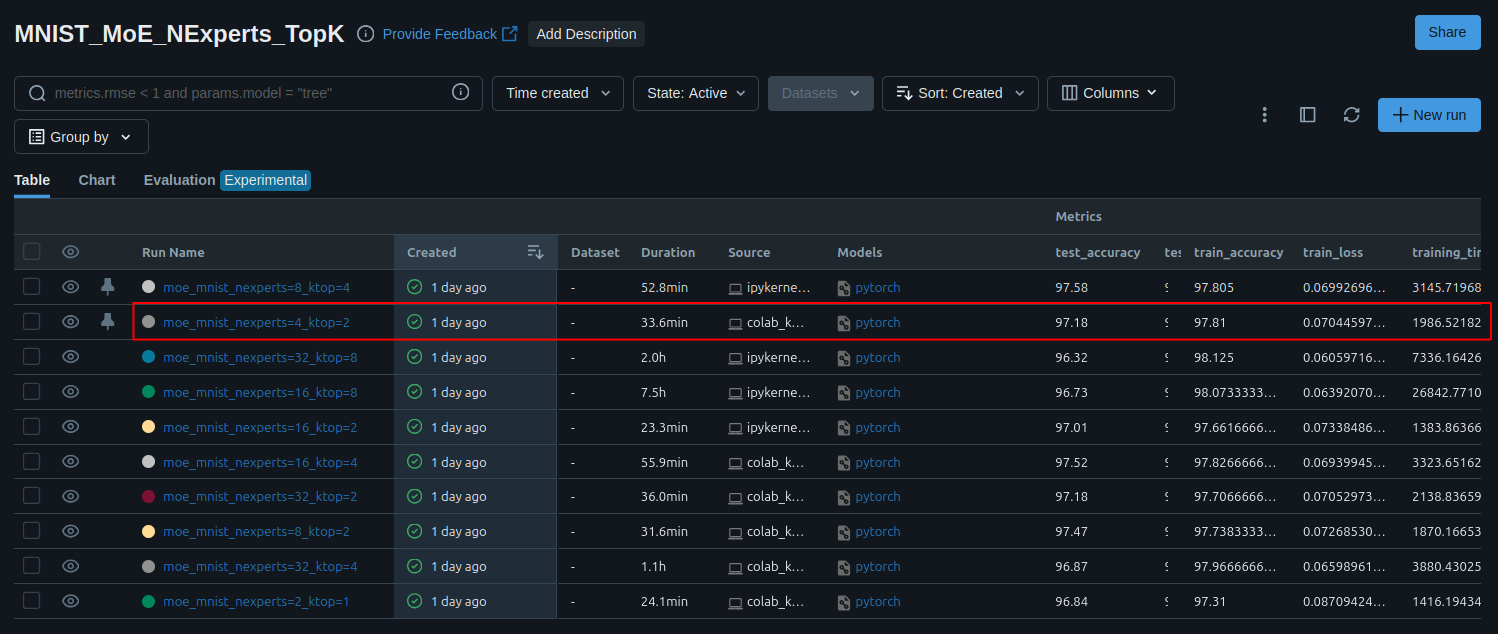
\includegraphics[width=0.6\textwidth]{images/experts_topk.png}
    \caption{Accuracy vs. Number of Experts and Top-k Selection}
    \label{fig:experts_topk}
\end{figure}

\begin{figure}[H]
    \centering
    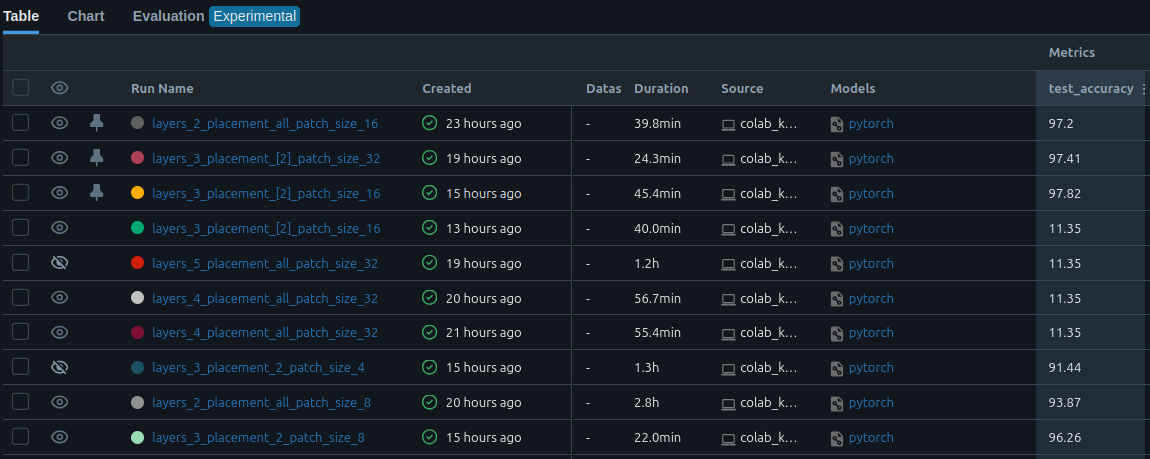
\includegraphics[width=0.6\textwidth]{images/patch_size.png}
    \caption{Accuracy vs. Patch Size}
    \label{fig:patch_size}
\end{figure}

\begin{figure}[H]
    \centering
    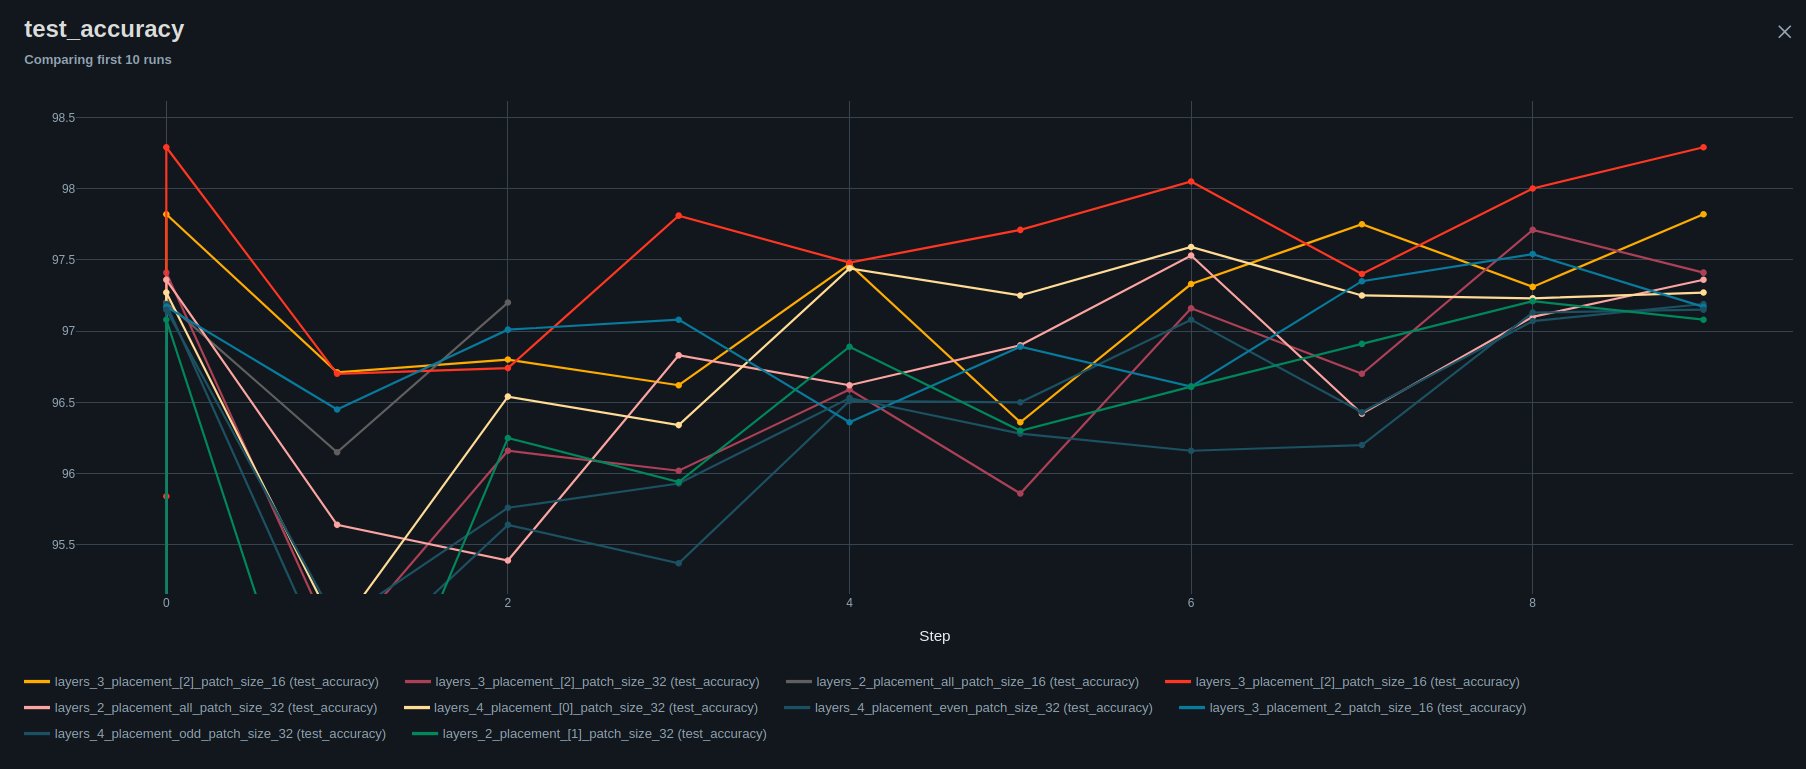
\includegraphics[width=0.6\textwidth]{images/layers_placement.png}
    \caption{Accuracy vs. Number of Layers and Expert Placement}
    \label{fig:layers_placement}
\end{figure}

\begin{figure}[H]
    \centering
    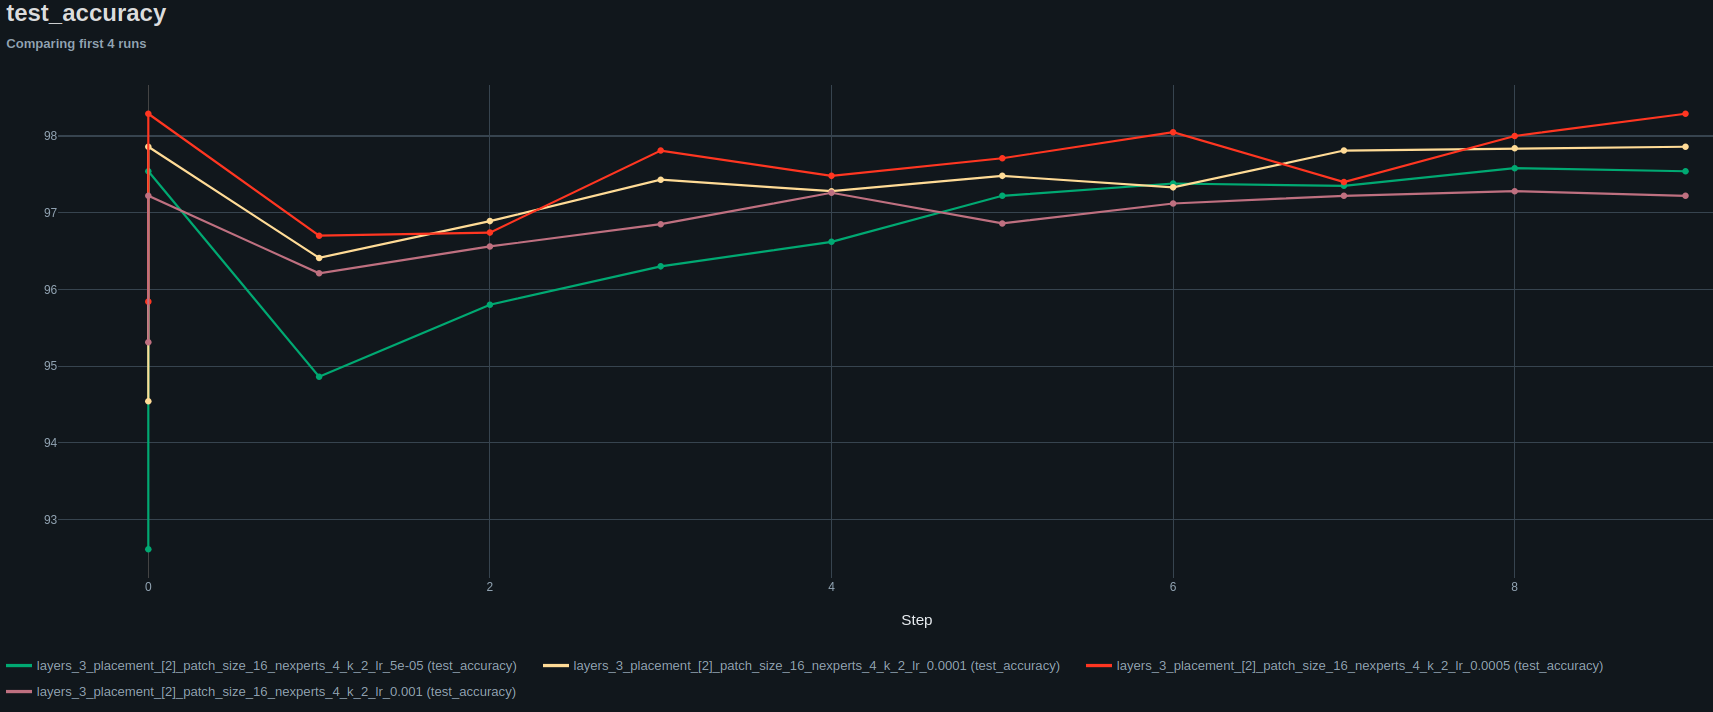
\includegraphics[width=0.6\textwidth]{images/learning_rate.png}
    \caption{Accuracy vs. Learning Rate}
    \label{fig:learning_rate}
\end{figure}

\begin{figure}[H]
    \centering
    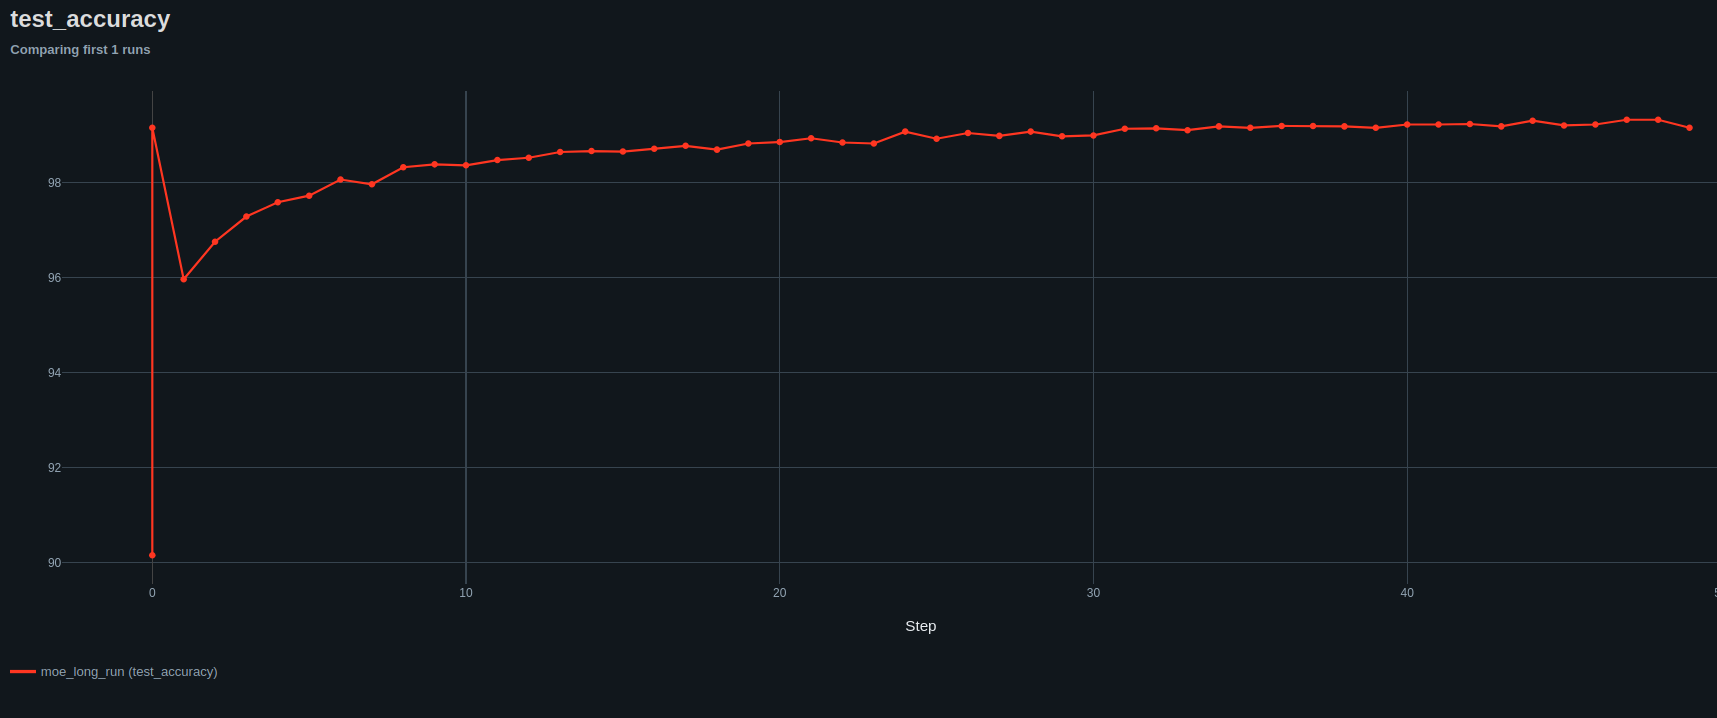
\includegraphics[width=0.6\textwidth]{images/long_run.png}
    \caption{Accuracy vs. Epochs (Long Run)}
    \label{fig:long_run}
\end{figure}

\begin{figure}[H]
    \centering
    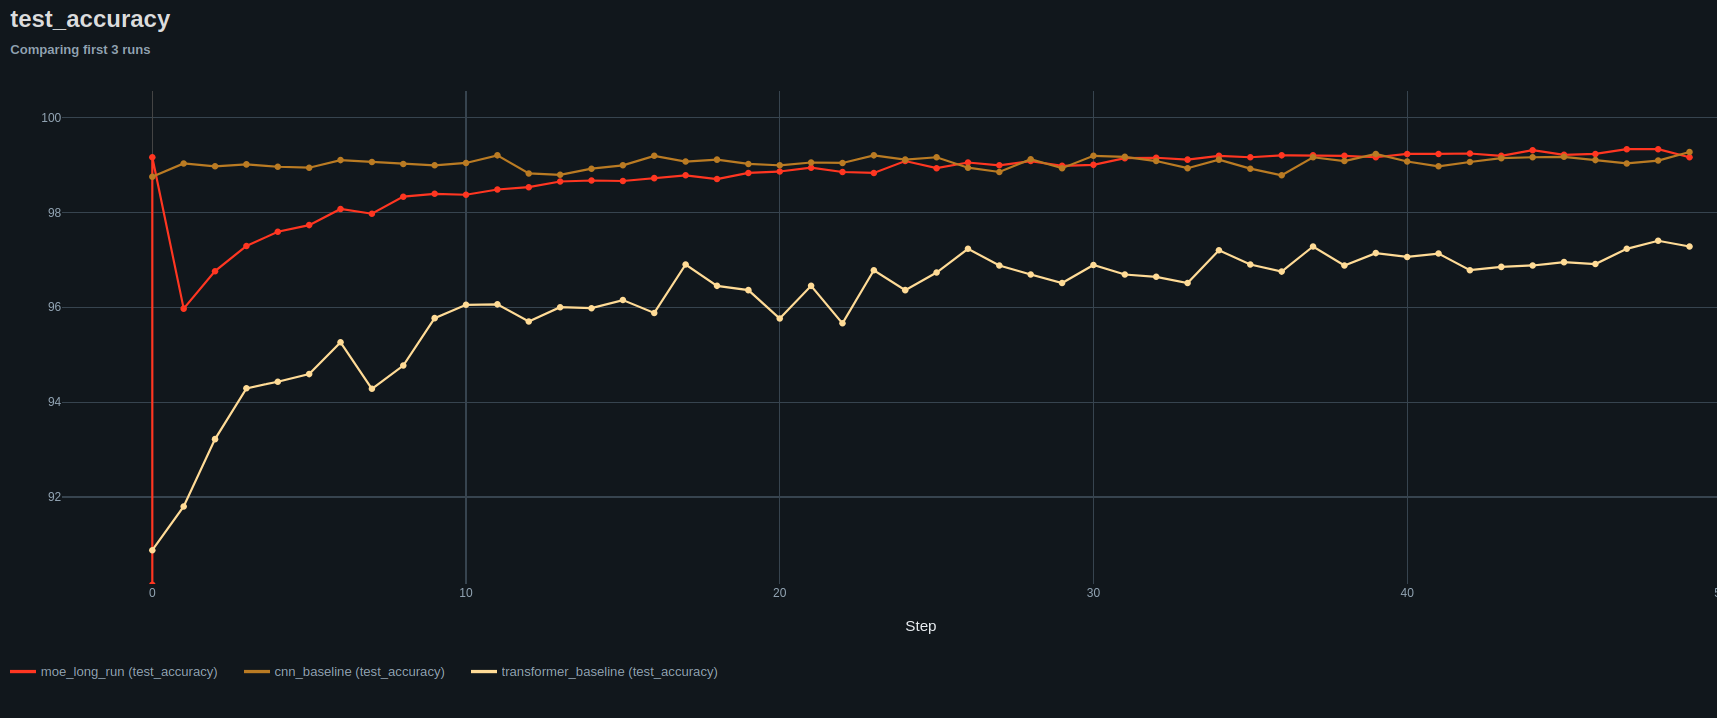
\includegraphics[width=0.6\textwidth]{images/baselines.png}
    \caption{Comparison of MoE Model with CNN and Standard Transformer}
    \label{fig:baselines}
\end{figure}

% --------------------------------------------

\section{References}

\renewcommand{\section}[2]{}%
%\renewcommand{\chapter}[2]{}% for other classes

% \bibliographystyle{plain}
\bibliographystyle{ieeetr}
\bibliography{references}

\end{document}